\documentclass{article}
\usepackage{graphicx}
\usepackage{listings}
\usepackage{ctex}
\usepackage{graphicx}
\usepackage[a4paper, body={18cm,22cm}]{geometry}
\usepackage{amsmath,amssymb,amstext,wasysym,enumerate,graphicx}
\usepackage{float,abstract,booktabs,indentfirst,amsmath}
\usepackage{array}
\usepackage{booktabs} %调整表格线与上下内容的间隔
\usepackage{multirow}
\usepackage{diagbox}
\usepackage{indentfirst}
\usepackage{bm}
\usepackage{fancyhdr}




\pagestyle{fancy}

\lhead{\bfseries \normalsize 学号:1952033\quad 姓名:侯雅玥 \quad 组员:廖宏 \\实验名称:负反馈放大电路的研究\quad 课程名称:电子技术实验\quad 专业:微电子科学与工程 } 
\rhead{}

\begin{document}

	\section{\zihao{4} 实验名称:负反馈放大电路的研究}
    \section{\zihao{4} 实验目的}
    \zihao {5} (1)研究负反馈对放大器各项性能指标的影响\par
	           (2)理解电路中引入负反馈的意义和方法\par
               (3)进一步熟悉放大电路中$A_u,f_L,f_H,$及$R_i,R_o$的测量方法\par
			   \section{\zihao{4} 实验原理}
			   反馈指将放大器输出端的信号(电压或电流)通过反馈网络按一定的方式回送到放大器的输入端,
			   并与输入信号一起参与输入端的控制,这个过程就是反馈,如图1所示为反馈放大器的方框图
			   \begin{figure}[h]
                \centering
                  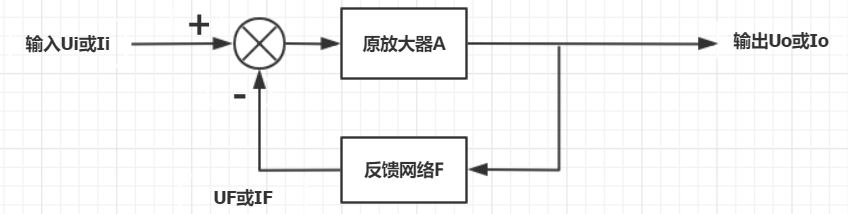
\includegraphics[width=12cm]{H:/电子技术试验/4-7/4-7-1.png}
                \caption{Figure example 1} 
              \end{figure}
			   根据反馈的极性不同,反馈可以分为正反馈和负反馈.正反馈引入的反馈信号增强输入信号的作用,
			   从而使放大电路的放大倍数得到提高;负反馈反馈信号削弱输入信号的作用,使放大倍数降低
			   在放大电路中,负反馈能提高电压放大
			   倍数的稳定性,减少非线性失真,抑制干扰,扩展通频带,改变输入、输出电阻等,但在一般多级放
			   大器中,应尽量避免和克服寄生反馈,防止寄生反馈给放大器带来负作用。
			   根据输出端反馈信号的采样方式,反馈又可分为电压负反馈(反馈网络并联接在输出端,反馈信号
			   正比于输出电压)及电流负反馈(反馈网络串联接在输出端,反馈信号正比于输出电流).从输入端看,
			   反馈信号$I_F$,与输入信号$I_i$并联相接的称为并联负反馈;反馈信号$U_F$,与输入信号$U_i$串联相接的称为串联
			   负反馈。本实验研究电压串联负反馈和电流串联负反馈对放大器电路性能的影响。\par
			   (1)负反馈使放大器的电压放大倍数下降,即
			   \begin{equation}
                \ A_{uf}=\frac{A_u}{1+A_{u}F}
			   \end{equation}
               \par
			       式中 $A_u$———无反馈时开环电压放大倍数;\par
			  \, \qquad $A_{u}F$———有反馈时闭环电压放大倍数;  \par
			  \, \qquad $F$———反馈系数。\par
			   由式(1)可知,$(1+A_{u}F)$越大,负反馈越强,当 $A_{u}F\gg1$时,上式可写成
               \begin{equation}
                \ A_{uF}\approx \frac{1}{F}
               \end{equation}
               \par
        	   即在深度负反馈情况下,电压放大倍数只与反馈网络有关,而与原放大器的电压放大倍数无关.\par
			   (2)负反馈展宽了放大器的通频带,即
               \begin{align}
                \ f_H&=(1+A_{u}F)f_H^{'} \\
                \ f_L&=\frac{f_L^{'}}{1+A_{u}F}
               \end{align}   
               \par     
               (3)负反馈提高了放大器电压增益的稳定性.加入负反馈后,稳定性的改善程度由放大
               倍数的相对变化量\par 表示:
               \begin{equation}\label{Delta}
                \ \frac{\varDelta A_{u}F}{A_{u}F}=\frac{\varDelta A_{u}}{A_u}\frac{1}{1+A_{u}F}
               \end{equation}
             
                由式\eqref{Delta}可以看出,引入负反馈后,增益的稳定度值减小,稳定性提高。\par
                (4)负反馈改善了放大器的非线性失真。\par
                (5)负反馈影响了输入电阻和输出电阻。\par
              负反馈对输入电阻的影响与反馈网络在放大器输入端的连接方式有关,而与输出端的连接方式无关,串联负
              反馈输入电阻增大到基本放大器的$(1+A_{u}F)$倍;并联负反馈则使输入电阻减小到基本放大器的$\frac{1}{1+A_{u}F}$倍。\par
              负反馈对输出电阻的影响与反馈网络在放大器输出端的取样方式有关,而与输入端连接方式无关,电压负反馈
              使放大器的输出电阻减小到基本放大器的$\frac{1}{1+A_{u}F}$倍,电流负反馈则使输出电阻增大到基本放大器的$(1+A_{u}F)$倍。\par

\section{\zihao{4} 实验电路}
电路图中,若将5和12连接,即接通$R_{f2}$则有1、2极极间反馈,若断开则无极间反馈\par
\begin{figure}[h]
	%\small
	\centering
	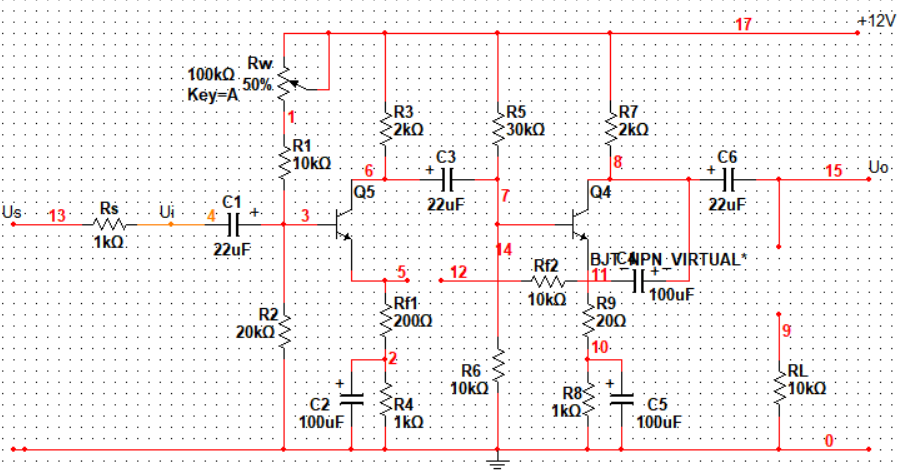
\includegraphics[width=16cm]{H:/电子技术试验/4-7/4-7-2.png}
	\caption{Figure example 2} \label{fig:aa}
\end{figure}
\section{\zihao{4} 实验内容及步骤}
\subsection {静态工作点的测量与研究}
(1)按照图2连接电路,断开$R_{f2}$,接通直流电源,调节$R_W$使$I_{C1}=2mA(U_{R3}=4V)$。记录$U_{CQ},U_{C2Q}$的数值。\par
(2)保持电路及输入电压不变,上下调节信号发生器的频率$f$使得此时的输出电压$U_o^{'}=0.707U_o$,此时的高低频率分别为$f_H,f_L$
	
\subsection{负反馈放大电路的数据测量}
\subsubsection{测量无反馈放大电路数据}
(1)输出电压及放大器放大倍数\par
断开$R_{f2}$,接通电源,在放大器的输入端加$f=1kHz$,的正弦信号,将双踪示波器接在$U_i$端,调节输入电压$U_s$,使$U_i$的有效值为5mV,测量此时的$U_o,U_s$的值,记录到表2\par
(2)接通负载$R_L$,测量有负载时的输出电压$U_{oL}$,计入表2\par
(3)$f_H,f_L$的测量\par
断开负载,保持电路及输入电压不变,上下调节信号发生器的频率$f$使得此时的输出电压$U_o^{'}=0.707U_o$,此时的高低频率分别为$f_H,f_L$\par
\subsubsection{测量有反馈放大电路数据}
(1)输出电压及放大器放大倍数\par
接通$R_{f2}$,接通电源,在放大器的输入端加$f=1kHz$,的正弦信号,将双踪示波器接在$U_i$端,调节输入电压$U_s$,使$U_i$的有效值为20mV,测量此时的$U_o,U_s$的值,记录到表2\par
(2)接通负载$R_L$,测量有负载时的输出电压$U_{oL}$,计入表2\par
(3)$f_H,f_L$的测量\par
断开负载,保持电路及输入电压不变,上下调节信号发生器的频率$f$使得此时的输出电压$U_o^{'}=0.707U_o$,此时的高低频率分别为$f_H,f_L$\par
\newpage
	\section{\zihao{4} 数据处理}

    \begin{table}[h]
        \centering  
        \begin{tabular}{c|c|c|c}
            \hline
                $I_{C1}$  &  $U_{R3}$    & $U_{C1Q}$     & $U_{C2Q}$   \\ \hline
                      2mA &   4V         & 8.01V         &7.66V        \\ \hline
        \end{tabular}
        \caption{静态工作点数据表}\label{SIGN}
        \end{table}
        
    \begin{table}[h]
        \centering  
        \begin{tabular}{c|c|c|c|c|c|c|c|c}
            \hline
            
                $U_s$   &  $U_i$    & $U_o$    & $f_L$  &  $f_H$    &  $R_i$                &  $R_o$          &  $A_u$  &  $U_{oL}$ \\ \hline
                5.30mV  &  5.00mV   & 1.57V    & 42Hz   &  300kHz   & \qquad \qquad \qquad  &  $1.98k\Omega$  &  314    &  1.31V    \\ \hline
                20.00mV &  21.74mV  & 857mV    & 49.3Hz &  1.445MHz & \qquad \qquad \qquad  &  $350\Omega$    &  43     &  828mV    \\ \hline
        \end{tabular}
        \caption{负反馈放大电路数据测量}\label{SIGN}
        \end{table}
        
	(1)计算输入输出电阻$R_i$与$R_o$\par
	有级间反馈时:
	\begin{align*}
		\ R_{i}&=\frac{U_i}{U_s-U_i}\times R_s=\qquad \quad k\Omega\\
		\ R_{o}&=(\frac{U_o}{U_{oL}}-1)\times R_L=1.98k\Omega\\
	\end{align*}
	无负载时:
	\begin{align*}
		\ R_{i}&=\frac{U_i}{U_s-U_i}\times R_s=\qquad \quad k\Omega\\
		\ R_{o}&=(\frac{U_o}{U_{oL}}-1)\times R_L=350\Omega\\
	\end{align*}
	(2)计算电压放大器的倍数
	有反馈时:
	\begin{equation*}
		\ A_{u}=\frac{U_{o}}{U_i}=314\\
	\end{equation*}
	无负载时:
	\begin{equation*}
		\ A_{u}=\frac{U_{o}}{U_i}=43\\
	\end{equation*}
	填入表格2
	

	\section{\zihao{4} 实验设备和器材}
	(1)双踪示波器             \qquad \qquad \qquad \qquad \qquad  \qquad           1台\par
	(2)函数信号发生器          \qquad  \qquad \qquad \qquad       \qquad           1台\par
	(3)直流稳压电源             \qquad \quad \qquad \qquad \qquad \qquad           1台\par
	(4)模拟电路实验箱            \qquad  \qquad \qquad \qquad\qquad                1台\par
	(5)万用表                   \qquad  \qquad \qquad \qquad \qquad \qquad \qquad  1只\par
	(6)三极管NPN9011、电阻器、电容器  \qquad                                        若干
\section{误差处理}
输入电阻的理论值
\begin{align*}
	\ R_{i0}&=R_2||(R_1+R_w)||(r_e+R_{f1})=\\
	\ \delta_{R_i} &=\frac{R_{i0}-R_i}{R_{i}}=\\
	\ R_{if}&=R_i \times (A_uF+1)=\\
	\ \delta_{R_{if}} &=\frac{R_{if0}-R_{if}}{R_{if}}=\\
\end{align*}
\par
输电出阻的理论值
\begin{align*}
	\ R_o&=R_7=2k\Omega\\
	\ \delta_{R_o} &=\frac{R_{o0}-R_o}{R_{o}}=1\%\\
	\ R_{of}&=R_o\times \frac{1}{A_uF+1}=318\Omega\\
	\ \delta_{R_{of}} &=\frac{R_{of0}-R_of}{R_{of}}=9.1\%
\end{align*}
\par
有负载的通频带
\begin{align*}
	\ f_{Lf0}&=f_L\times\frac{1}{1+A_uF}=5.61Hz\\
	\ f_{Hf0}&=f_H\times(1+A_uF)=1.570MHz\\
	\ \delta_{f_{Hf}} &=\frac{f_{Hf0}-f_{Hf}}{R_{Hf}}=7.6\%\\
\end{align*}
\par 
(1)其中有负载时,低频$f_L$误差较大,但是在实际试验中,频率过低的情况下,示波器采集不到清晰的信号,因此在测试截止前时的频率被认为是低频$f_H$\par
(2)误差可能是器件老化造成。\par
\newpage
\section{结论}
馈对放大器电路性能的影响。\par
			   (1)负反馈使放大器的电压放大倍数下降,即
			   \begin{equation*}
                \ A_{uf}=\frac{A_u}{1+A_{u}F}
			   \end{equation*}
               \begin{equation*}
                \ A_{uF}\approx \frac{1}{F}
               \end{equation*}
               \par
			   (2)负反馈展宽了放大器的通频带,即
               \begin{align*}
                \ f_{Hf}&=(1+A_{u}F)f_H \\
                \ f_{Lf}&=\frac{f_L}{1+A_{u}F}
               \end{align*}   
               \par
                (3)负反馈影响了输入电阻和输出电阻。\par
            串联负反馈输入电阻增大到基本放大器的$(1+A_{u}F)$倍,电压负反馈使放大器的输出电阻减小到基本放大器的$\frac{1}{1+A_{u}F}$倍,\par

\section{思考题}
(1)在两级电压串联负反馈电路中,若反馈电压取自$T_2$的发射极,会有什么结果?\par
若反馈电压取自$T_2$的发射极,则为并联-并联分馈电路,有如下结果:
\begin{align*}
	\ R_{of}&=\frac{R_o}{(1+A_{u}F)}\\
	\ R_{if}&=\frac{R_i}{(1+A_{u}F)}\\
	\ A_{uf}&=\frac{A_u}{(1+A_{u}F)}\\
   \end{align*}  
   \par
(2)反馈电路为什么能改善放大器的波形失真?\par
因为利用负反馈降低增益灵敏度的作用,就能使放大器在更宽频率范围内维持增益不变,从而有效地扩展了放大器的通频带。\par
(3)如何判断电路是否有自激振荡?有自激振荡时采取哪些措施?\par
如果在放大器的输入端不加输入信号,输出端仍有一定的幅值和频率的输出信号,这种现象就是自激振荡。\par
可以采用频率补偿(又称相位补偿)的方法,消除自激振荡。常用补偿方法有电容滞后补偿,即在放大电路中选择时间常数最大的回路内对地并联一个小电容,这样当相移处于180度时,其高频放大倍数幅值下降到0以下。\par


\end{document}

